%ERGEBNISSE

\chapter{Bibtex, Citavi und Zitieren} \label{kap:bibtex}
Diese LaTeX-Vorlage verwendet Bibtex zur einfachen Darstellung eines Literaturverzeichnisses.

Es gibt verschiedene Editoren f�r Bibtex Dateien, z.B. JabRef.

Wird mit Citavi gearbeitet, so kann die Literatur automatisch in eine Bibtex-Datei geschrieben werden. \\

Daf�r auf Datei -> Exportieren

\begin{figure}[h]
	\centering
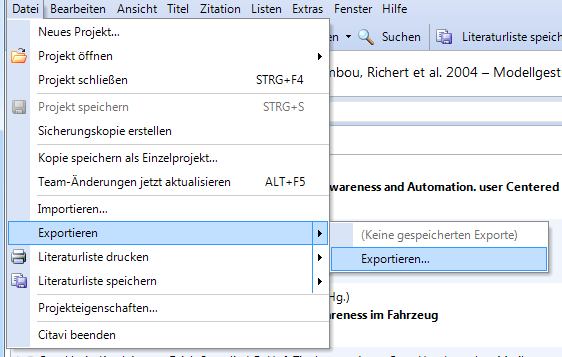
\includegraphics[width=12cm]{img/bib1.png}
\caption{\textit{Exportieren}}
\label{fig:bib1}
\end{figure} 

Im n�chsten Fenster auf "Alle XX Titel in diesem Projekt" und "Weiter".\\

Anschlie�end "BibTeX" anw�hlen und "Weiter".

\begin{figure}[!ht]
	\centering
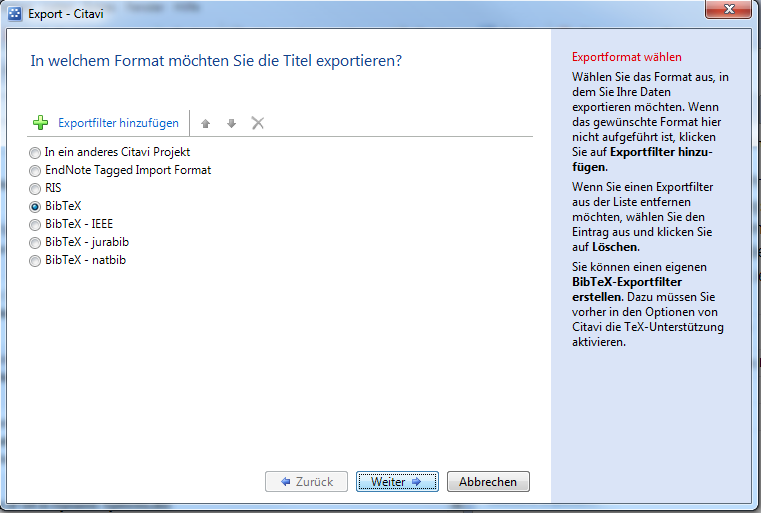
\includegraphics[width=13cm]{img/bib2.png}
\caption{\textit{Fomart zum Exportieren}}
\label{fig:bib2}
\end{figure} 

Jetzt die entsprechende *.bib Datei ausw�hlen. Diese sollte in dem Projektordner liegen und Bibtex.bib hei�en. F�r einen anderen Ort oder Dateinamen muss "$\backslash$bibliography\{Bibtex\}" im "Studienarbeit.tex" entsprechend angepasst werden.
Au�erdem einen Haken bei "Bibtex-Datei aktualisieren".

\begin{figure}[!ht]
	\centering
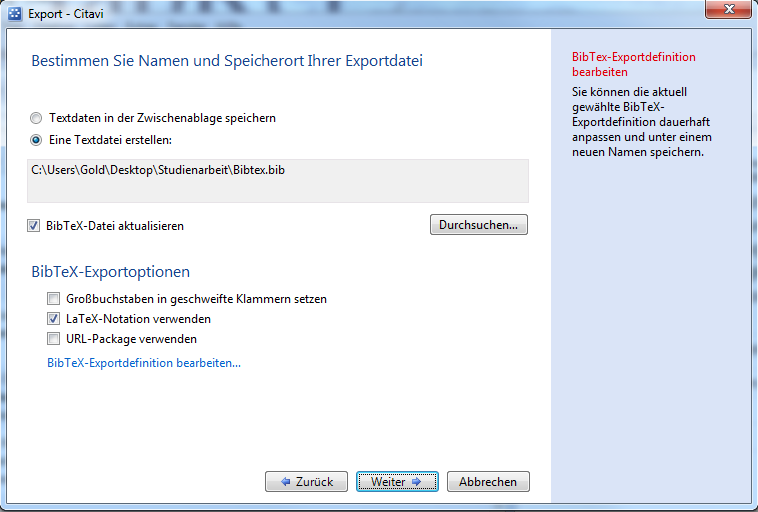
\includegraphics[width=13cm]{img/bib3.png}
\caption{\textit{Datei ausw�hlen}}
\label{fig:bib3}
\end{figure} 

Im n�chsten Fenster der Exportvorlage einen Namen geben und einen Haken bei "Automatisch exportieren beim Speichern" setzen. 

\begin{figure}[ht]
	\centering
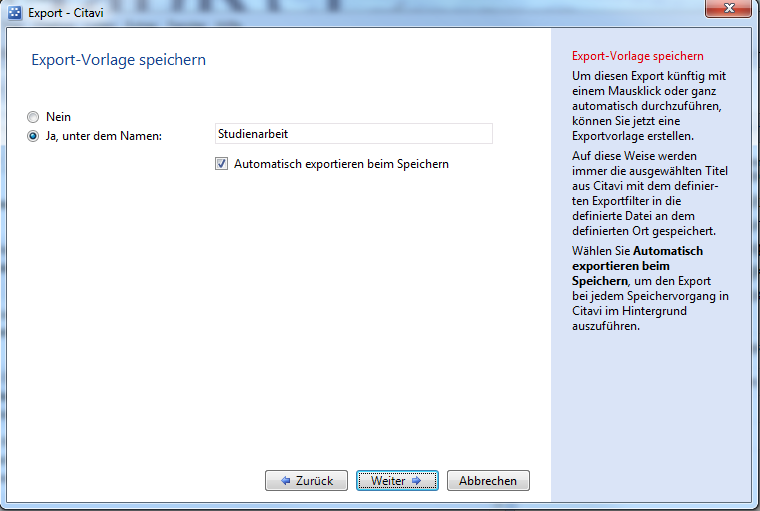
\includegraphics[width=13cm]{img/bib4.png}
\caption{\textit{Automatisch aktualisieren}}
\label{fig:bib4}
\end{figure} 

Bei jeder �nderung in Citavi aktualisiert sich die Bibtex-Datei automatisch mit und ist somit immer auf dem aktuellstem Stand. 

Die gesamte in Citavi gespeicherte Literatur steht nun zum zitieren bereit und es kann mit "$\backslash$cite\{Name.Jahr\}" eine Literaturangabe gesetzt werden. Damit alle Zitate und Seitenzahlen stimmen, muss das Projekt am Ende mehrfach kompiliert werden.\\

Beispiel:

So sagte \cite{Mustermann.2012}, dass... bzw. "Ich bin klug" \citep{Mustermann.2012}.
